% !TeX encoding = UTF-8
% !TeX spellcheck = es_ES
\documentclass[12pt]{article}
\usepackage{fullpage}
\usepackage[utf8]{inputenc}
\usepackage{pict2e}
\usepackage{amsmath}
\usepackage{enumitem}
\usepackage{eurosym}
\usepackage{mathtools}
\usepackage{amssymb, amsfonts, latexsym, cancel}
\setlength{\parskip}{0.3cm}
\usepackage{graphicx}
\usepackage{fontenc}
\usepackage{setspace}
\usepackage{pgfplots}
\usepackage{adjustbox}
\setstretch{1.5}
\usepackage{bold-extra}
\usepackage{subcaption}
\usepackage{wasysym}
\graphicspath{ {images/} }
\usepackage{tcolorbox}
\usepackage{xcolor, colortbl}
\usepackage{wrapfig}
\usepackage{empheq}
\usepackage{array}
\usepackage{parskip}
\usepackage{arydshln}
\renewcommand*\contentsname{\color{black}Índice} 
\usepackage{array, multirow, multicol}
\definecolor{blueice}{rgb}{.2, .6, .8}
\definecolor{lightblue}{HTML}{007AFF}
\usepackage{color}
\usepackage{etoolbox}
\usepackage{listings}
\usepackage{mdframed}
\setlength{\parindent}{0pt}
\usepackage{underscore}
\usepackage{hyperref}
\usepackage{tikz}
\usetikzlibrary{shapes, positioning, patterns}
\usepackage{tikz-qtree}
\usepackage{biblatex}
\usepackage{pdfpages}
\usepackage{pgfplots}
\usepackage{pgfkeys}
\addbibresource{biblatex-examples.bib}
\usepackage[a4paper, left=1cm, right=1cm, top=1cm,
bottom=1.5cm]{geometry}
\everymath{\displaystyle}
\usetikzlibrary{decorations.pathreplacing}
\usepackage{titlesec}
\setlength{\fboxrule}{1.5pt}
\renewcommand{\arraystretch}{1.5}
\newcommand{\bboxed}[1]{\fcolorbox{lightblue}{lightblue!10}{$#1$}}

\begin{document}
\section*{Cálculo I}

$\underset{\displaystyle\downarrow}{P(n)}\qquad n\ge 1$

La fórmula depende de $n$

\textcolor{olive}{\texttt{\# Psuedocódigo}}

\texttt{for n=1 to n=100,000}\\

\hrule

$\left.\begin{array}{l}
	P(1) \text{\textcolor{lightblue}{ elemento mínimo}}\\
	P(n)\longrightarrow P(n+1)
\end{array}\right\}$Suponemos que $P(n)$ es cierta. Demostraremos $P(n+1) \rightarrow P(n)$ cierta $\forall n\in \mathbb{N}$

Supongamos por reducción al absurdo

$A=\{n\in\mathbb{N}:P(n) \text{ es falsa}\}\neq\varnothing$

Suponiendo lo contrario de lo que quiero demostrar se llega a una contradicción.

$A\subset\mathbb{N}$

$\exists n_0\in A$ elemento mínimo

Si el elemento mínimo es falso $\longrightarrow$ todos los anteriores son verdaderos
\begin{itemize}[label=\color{red}\textbullet, leftmargin=*]
	\item \color{lightblue}Ejercicio
\end{itemize}
{\color{lightblue} Establecer la igualdad \[ 1+2+3\cdots+n=\dfrac{n(n+1)}{2} \] para $n\ge1$ (también lo podemos indicar de la forma $n\in\mathbb{N}$)}

$P(n)=\dfrac{n+1}{2}\cdot n$

\begin{itemize}[leftmargin=*]
	\item $n=1$
	
	$P(1)=\dfrac{1+1}{2}\cdot 1=1\textcolor{lightblue}{\checked}$
	
	\item $n=2$
	
	$P(2)=\dfrac{2+1}{2}\cdot 2=3\textcolor{lightblue}{\checked}$
	
	\item Supongamos que $P(n)$, es decir, $1+2+\cdots+n=\dfrac{n(n+1)}{2}$ y queremos demostrar que $P(n+1)$, es decir,  $1+2+\cdots+n+(n+1)=\dfrac{(1+(n+1))}{2}\cdot(n+1)$
	
	\item[$\longrightarrow$] Demostración
	
	$\begin{array}{ll}
		\underbrace{1+2+\cdots+n}_{P(n)}+(n+1) & =\dfrac{(1+n)}{2}\cdot+(n+1)\\
		&=\dfrac{(1+n)\cdot n+2(n+1)}{2}\\
		&=\dfrac{(1+n)\cdot(n+2)}{2} \textcolor{lightblue}{\checked}
	\end{array}$
\end{itemize}

\begin{wrapfigure}[6]{r}{0.4\linewidth}
	\begin{tikzpicture}% function
		\begin{axis}[ymin=-1, xmin=-1, ymax=4, xmax=4, axis lines=center]
			\addplot[lightblue, samples=150, domain=0:4] {sqrt(x)};
		\end{axis}
	\end{tikzpicture}
\end{wrapfigure}
Por la propiedad transitiva, $a<b$:

$a>0$

$a<b\rightarrow a^2< ab\rightarrow\sqrt{a^2}<\sqrt{ab}\rightarrow a=|a|<\sqrt{ab}$


$(a-b)^2>0\rightarrow a^2-2ab+b^2>0\rightarrow a^2+b^2>2ab\rightarrow a^2+b^2+2ab>2ab+2ab;~a^2+b^2+2ab>4ab,~(a-b)^2>4ab\rightarrow\dfrac{(a+b)^2}{4}>ab\rightarrow \dfrac{a+b}{2}=\sqrt{ab}$

$(a+b)^n=\sum_{i=0}^{n}\binom{n}{i}a^i\cdot b^{n-1}$

\begin{align*}
	(a+b)^n\cdot(a+b)&=\left(\sum_{i=0}^{n}\binom{n}{i}a^i\cdot b^{n-i}\right)(a+b)\\
	&=\left(\binom{n}{i}b^n+\binom{n}{1}a\cdot b^{n-1}+\binom{n}{2}a^2\cdot b^{n-2}+\cdots+\binom{n}{n}a^n\right)\cdot(a+b)\\
	&=a\cdot b^n+\binom{n}{1}a\cdot b^{n-1}+\cdots+\binom{n}{n}a^n+b^{n+1}+\binom{n}{1}a\cdot b^n+\binom{n}{2}a^2\cdot b^{n-1}+\cdots+\binom{n}{n}a^n\cdot b
\end{align*}

\begin{align*}
	\binom{n}{k}\cdot\dfrac{1}{n^k}=\dfrac{n!}{k!(n-k)!}\cdot\dfrac{1}{n^k}&=\dfrac{1}{k!}\cdot\dfrac{n\cdot(n-1)\cdot(n-2)\cdot~\cdots~\cdot\overset{n-(k-1)}{(n-k+1)}\cdot\cancel{(n-k)!}}{\cancel{(n-k)!}\cdot\underbrace{n\cdot n\cdot n\cdot~\cdots~\cdot n}_{k\text{ veces}}}\\
	&=\dfrac{1}{k!}\cdot1\cdot\left(1-\dfrac{1}{n}\right)\cdot\left(1-\dfrac{2}{n}\right)\cdot~\cdots~\cdot\left(1-\dfrac{(k-1)}{n}\right)<\dfrac{1}{k!}
\end{align*}

$\left(1+\dfrac{1}{n}\right)^n\le\sum_{k=0}^{n}\dfrac{1}{2^{k-1}}=1+\sum_{k=1}^{n}\dfrac{1}{2^{k-1}}$

\begin{wrapfigure}[4]{r}{0.5\textwidth}
	\begin{tikzpicture}[baseline=(current bounding box.center)]% function
		\begin{axis}[xlabel=$n$,ylabel=$f(n)$, ymin=-1, xmin=-1, axis lines=center]
			\addplot[domain=0:4.5, lightblue, samples=150] {(x^2+1)/5};
		\end{axis}
	\end{tikzpicture}
\end{wrapfigure}

\pagebreak[4]

$\underbrace{\begin{array}{l}
		b^*=\min\{\text{lista 1}\}\\
		a^*=\max\{\text{lista 1}\}\\
		\{a_1,a_2,\hdots,a_{n_0-1},a_{n_0},a_{n_0+1},\hdots\}\in(l-\varepsilon, ~l+\varepsilon)
\end{array}}_{\text{lista 1}}$

\begin{tikzpicture}	
	\draw (0,0) -- (9,0) node[right] {$x_{n+1}>x_n$};
	\foreach \x in {1,2,...,8}{
	\draw (\x,-0.25) -- (\x,0.25);
	};
\end{tikzpicture}

Supremo $=\max\{a,~l+\varepsilon\}$

$\lim_{n\to\infty}x_n=l$ si $\forall\varepsilon>0\exists n_0\in\mathbb{N}:|x_n-l|<\varepsilon$

$|x_m-x_n|<\varepsilon$ 

$\begin{array}{l}
	x_1=\sqrt{a}\\
	x_2=\sqrt{a+\sqrt{a}}\\
	x_3=\sqrt{a+\sqrt{a+\sqrt{a}}}\\
	x_{n+1}=\sqrt{a+x_n}
\end{array}$

\textcolor{lightblue}{\underline{Sucesiones de números reales}}

\begin{itemize}[label=\color{red}\textbullet, leftmargin=*]
	\item \color{lightblue}Definición
\end{itemize}
$\lim_{n\to\infty}a_n=l$ si $\forall\varepsilon>0\exists n_0\in\mathbb{N}$: si $n\ge n_0\rightarrow\dfrac{|x_n-l|<\varepsilon}{|x_m-x_n|<\varepsilon}$
\begin{itemize}[label=$\longrightarrow$]
	\item Cauchy
	\item Convergente $\Rightarrow$ acotado
	\item Creciente y acotada superior $\Rightarrow$ convergente
	\item Contractiva
	\item Subsecciones
	\item Equivalencias $\Rightarrow$ Stolz
	\item {\Large e}
	\item Teoría
\end{itemize}
\begin{itemize}[label=\color{red}\textbullet, leftmargin=*]
	\item \color{lightblue}Ejercicios de práctica 1
\end{itemize}
\textcolor{red}{1)}
\begin{enumerate}[label=\color{red}\alph*)]
	\item $\textcolor{lightblue}{a_n=2+0.1^n}=2$
	\item $\textcolor{lightblue}{}$
	\item $\textcolor{lightblue}{\lim_{n\to\infty}\dfrac{(-1)^n\sqrt{n}\sin(n^n)}{n+1}}\overset{n+1\equiv n}{=}\lim_{n\to\infty}\dfrac{(-1)^nn^{\frac{1}{2}}\sin(n^n)}{n}=\lim_{n\to\infty}\dfrac{\overbrace{(-1)^n}^{\{-1,1\}}\cdot\overbrace{\sin(x^n)}^{[-1,1]}}{n^{\frac{1}{2}}}=0$
	
	\item $\textcolor{lightblue}{\lim_{n\to\infty}} \left( n-1 \right) \sqrt{n+a}\sqrt{n+b} = n \cdot \left(1-\sqrt{\dfrac{(n+a)(n+b)}{n^2}}\right) = \lim_{n\to\infty} n \cdot \underbrace{\left(1-\left(\underbrace{\left(1+\dfrac{a}{n}\right)\cdot\left(1+\dfrac{b}{n}\right)}_{1+\frac{b}{n}+\frac{a}{n}+\frac{ab}{n^2}}\right)\right)^{\frac{1}{2}}}_{-\frac{1}{2}\cdot\left(\frac{b+a}{n}+\frac{ab}{n^2}\right)} = \lim_{n\to\infty} n \cdot \left(-\frac{1}{2}\cdot\left(\frac{b+a}{n}+\frac{ab}{n^2}\right)\right) = \lim_{n\to\infty} -\frac{1}{2} \left(b+a+\frac{ab}{n}\right) = -\frac{ab}{2}$

	
	$(a+a_n)^\alpha-1\equiv\alpha a_n\quad(a_n\rightarrow 0)$
	\item $\textcolor{lightblue}{\lim_{n\to\infty}\sqrt[n]{a^n+b^n}=}\lim_{n\to\infty}{\Large \mathrm{e}}^{\frac{1}{n}\ln(a^n+b^n)}=\left\{\lim_{n\to\infty}\dfrac{a^n}{b^n}=\dfrac{a^{n+1}-a^n}{b^{n+1}-b^n}\right\}={\Large \mathrm{e}}^{\ln(a)}$
	
	$-$ Criterio de Stolz $\longrightarrow \lim_{n\to\infty}\dfrac{\ln(a^n+b^n)}{n}=\lim_{n\to\infty}\dfrac{\ln(a^{n+1}+b^{n+1})-\ln(a^n+nb^n)}{\underbrace{n+1}-n}=$
	
	$\lim_{n\to\infty}\ln\left(\dfrac{a^{n+1}-b^{n}+1}{a^n+b^n}\right)=\lim_{n\to\infty}\ln\left(\dfrac{a^{n+a}\cdot \left(1+\left(\dfrac{b}{a}\right)^{n+1}\right)}{a^n\cdot\left(1+\left(\dfrac{b}{a}\right)^n\right)}\right)$
	
	\item $\lim_{n\to\infty}(-1)^n\cdot\left(1-\frac{1}{n}\right)$ No existe
	\item $\lim_{n\to\infty}\dfrac{\sin(n)}{n}=0$
	\item $\textcolor{lightblue}{\lim_{n\to\infty}\left(-\dfrac{1}{2}\right)^n=}0$
	\item $\textcolor{lightblue}{\lim_{n\to\infty}\left(\dfrac{n}{n+1}\right)^n=}\lim_{n\to\infty}\left(1+\dfrac{1}{-(n+1)}\right)^{\frac{-(n+1)}{-(n+1)}\cdot n}={\Large\mathrm{e}}^{-1}$
	
	$\lim_{n\to\infty}{\Large\mathrm{e}}^{n\ln\left(1-\frac{1}{n+1}\right)}=\lim_{n\to\infty}{\Large\mathrm{e}}^{n\cdot-\frac{1}{n+1}}={\Large\mathrm{e}}^{-1}$
	
	\item $\textcolor{lightblue}{\lim_{n\to\infty}\left(1-\dfrac{1}{n^2}\right)^n=}\lim_{n\to\infty}{\Large\mathrm{e}}^{n\ln\left(1-\frac{1}{n^2}\right)}=\lim_{n\to\infty}{\Large\mathrm{e}}^{-\frac{n}{n^2}}={\Large\mathrm{e}}^0=1$
	\item $\textcolor{lightblue}{\lim_{n\to\infty}\sqrt[n]{n^2}}\longleftarrow$ Stolz
	\item $\textcolor{lightblue}{\lim_{n\to\infty}(n+4)^{\frac{1}{n+4}}}$
	\item $\textcolor{lightblue}{\lim_{n\to\infty}\left(\dfrac{1}{n}\right)^{\frac{1}{\log(n)}}=}{\Large\mathrm{e}}^{\frac{1}{n}}$
\end{enumerate}

\textcolor{red}{5)} \textcolor{lightblue}{Demuestre que si $0<a<2$ entonces $a<\sqrt{2a}<2$}

$a<2\xrightarrow[a>0]{}a^2<2a\xrightarrow[f(x)=\sqrt{x}\text{creciente}]{}\sqrt{a^2}<\sqrt{2a}\xrightarrow[\sqrt{a^2}=|a|=a]{}a<\sqrt{2a}$

$a<2\longrightarrow 2a<4\xrightarrow[f(x)=\sqrt{x}]{}\sqrt{2a}<\sqrt{4}=2$

\textcolor{red}{b) }\textcolor{blue}{$\{\overset{a_1}{\sqrt{2}},\overset{\sqrt{2a_1}}{\sqrt{2\sqrt{2}}},\overset{\sqrt{2a_2}}{\sqrt{2\sqrt{2\sqrt{2}}}}, \hdots\}$}

$a_{n+1}=\sqrt{2a_n}$

$a=\boxed{\sqrt{2}}<2$

{$\renewcommand{\arraystretch}{0.8}\begin{array}{rcl}
	\sqrt{2a} & > & a\\
	\downarrow & &\downarrow\\
	\sqrt{2} & & \sqrt{2}\\
	\sqrt{2\sqrt{2}} & > &\sqrt{2}
\end{array}\qquad x_n\le\sqrt{2x_n}\qquad x_{n+1}=\sqrt{2x_n}$, monótona creciente}

$x_{n+1}\ge x_n$

$x_1=\sqrt{2}\qquad x_2=\sqrt{2\sqrt{2}}$

$x_n\ge x_{n-1}$ inducción \boxed{x_{n+1}\ge x_n}

\boxed{x_{n+1}=\sqrt{2x_{n}}\ge\sqrt{2x_{n-1}}=x_n}

Acotada superiormente 

$x_n\le2\qquad x_1=\sqrt{2}<2$

$x_{n+1}=\sqrt{2x_n}<2$ \textcolor{lightblue}{(Desigualdad apuntada)}

\textcolor{red}{c)} \textcolor{blue}{$x_{n+1}=\sqrt{2x_n}$}

$\lim_{n\to\infty}x_{n+1}=\lim_{n\to\infty}\sqrt{2x_n}$

{\renewcommand{\arraystretch}{0.8}$\begin{array}{ll}
	l=\sqrt{2l}= & l^2=2l\\
	 & l^2-2l=0\longrightarrow l(l-2)=0\left\{\begin{array}{l}
		\cancel{l=0}\\
		l=2
	\end{array}\right.
\end{array}$}

\textcolor{red}{6)}\textcolor{lightblue}{$\underset{\displaystyle x_{n+1}=\sqrt{1+x_n}}{x_1=1}$}

Monótona creciente y acotada superiormente

\underline{Monóntona creciente} $\qquad x_{n+1}>x_n$

$\left.\begin{array}{l}
	x_2=\sqrt{2}\\
	x_1=1
\end{array}\right\}x_2\ge x_1$

\begin{wrapfigure}[3]{r}{0.3\linewidth}
	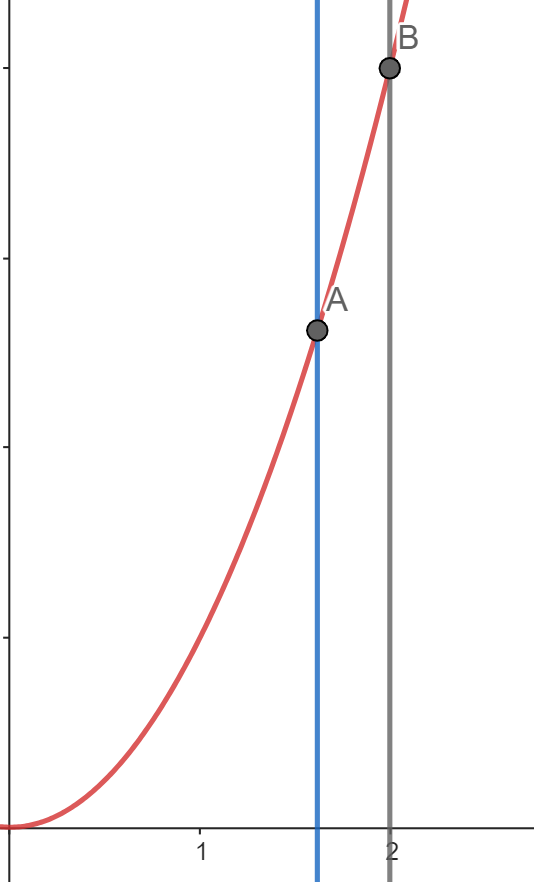
\includegraphics[scale=1.5]{imagenes/grafica2 29-09}
\end{wrapfigure}

\underline{Inducción:} suponemos que $x_n\ge x_{n+1}$ y queremos que $x_{n+1}\ge x_n$

$x_{n+1}=\sqrt{1+x_n}\ge \sqrt{1+x_n}=x_n$

\boxed{x_n\le k}

$x_{n+1}\ge x_n$

$\begin{array}{r}
		\underbrace{\sqrt{1+x_n}_{0}}\ge \underbrace{x_n}_{0}\longrightarrow(1+x_n)\ge x_n^2\\
		x_n^2-x_n-1\le0
	x_{n}=\dfrac{1\pm\sqrt{1+4}}{2}\longrightarrow x_n\le \dfrac{1+\sqrt{5}}{2}
\end{array}$\qquad



\textcolor{red}{9)}

$a_1=\alpha>0\qquad a_n>0$

$a_{n+1}=\dfrac{4a_n^2}{1+a_n^2}\qquad n\ge 1$

\textcolor{red}{a)} \textcolor{blue}{$x>0$}

$\boxed{\dfrac{4x^2}{1+4x^2}\le x}\xLeftrightarrow{x>0}\dfrac{4x}{1+4x^2}\le 1\xLeftrightarrow{1+4x^2>0}4x\le 4x^2+1\Longleftrightarrow 4x^2-4x+1\ge 0\Longrightarrow (2x-1)^2\ge0$

\textcolor{red}{b) }\textcolor{blue}{$a_{n+1}\le a_n$}

\textcolor{red}{c) }\textcolor{blue}{$\alpha\ge \dfrac{1}{2}\Longrightarrow a_n\ge\dfrac{1}{2}$}

$a_n\ge 0$

$a_{n+1}=\dfrac{4a_n^2}{1+4a_n^2}$

$a_{n+1}=\dfrac{4a_{n}^2}{1+4a_n^2}\Longleftrightarrow\dfrac{8a_n^2}{1+4a_n^2}\ge 1\Longleftrightarrow 8a_n^2\ge 1+4a_n^2\Longleftrightarrow 4a_n^2\ge 1\Longleftrightarrow a_n^2\ge\dfrac{1}{4}\Longleftrightarrow\boxed{a_n\ge\dfrac{1}{2}}$
 

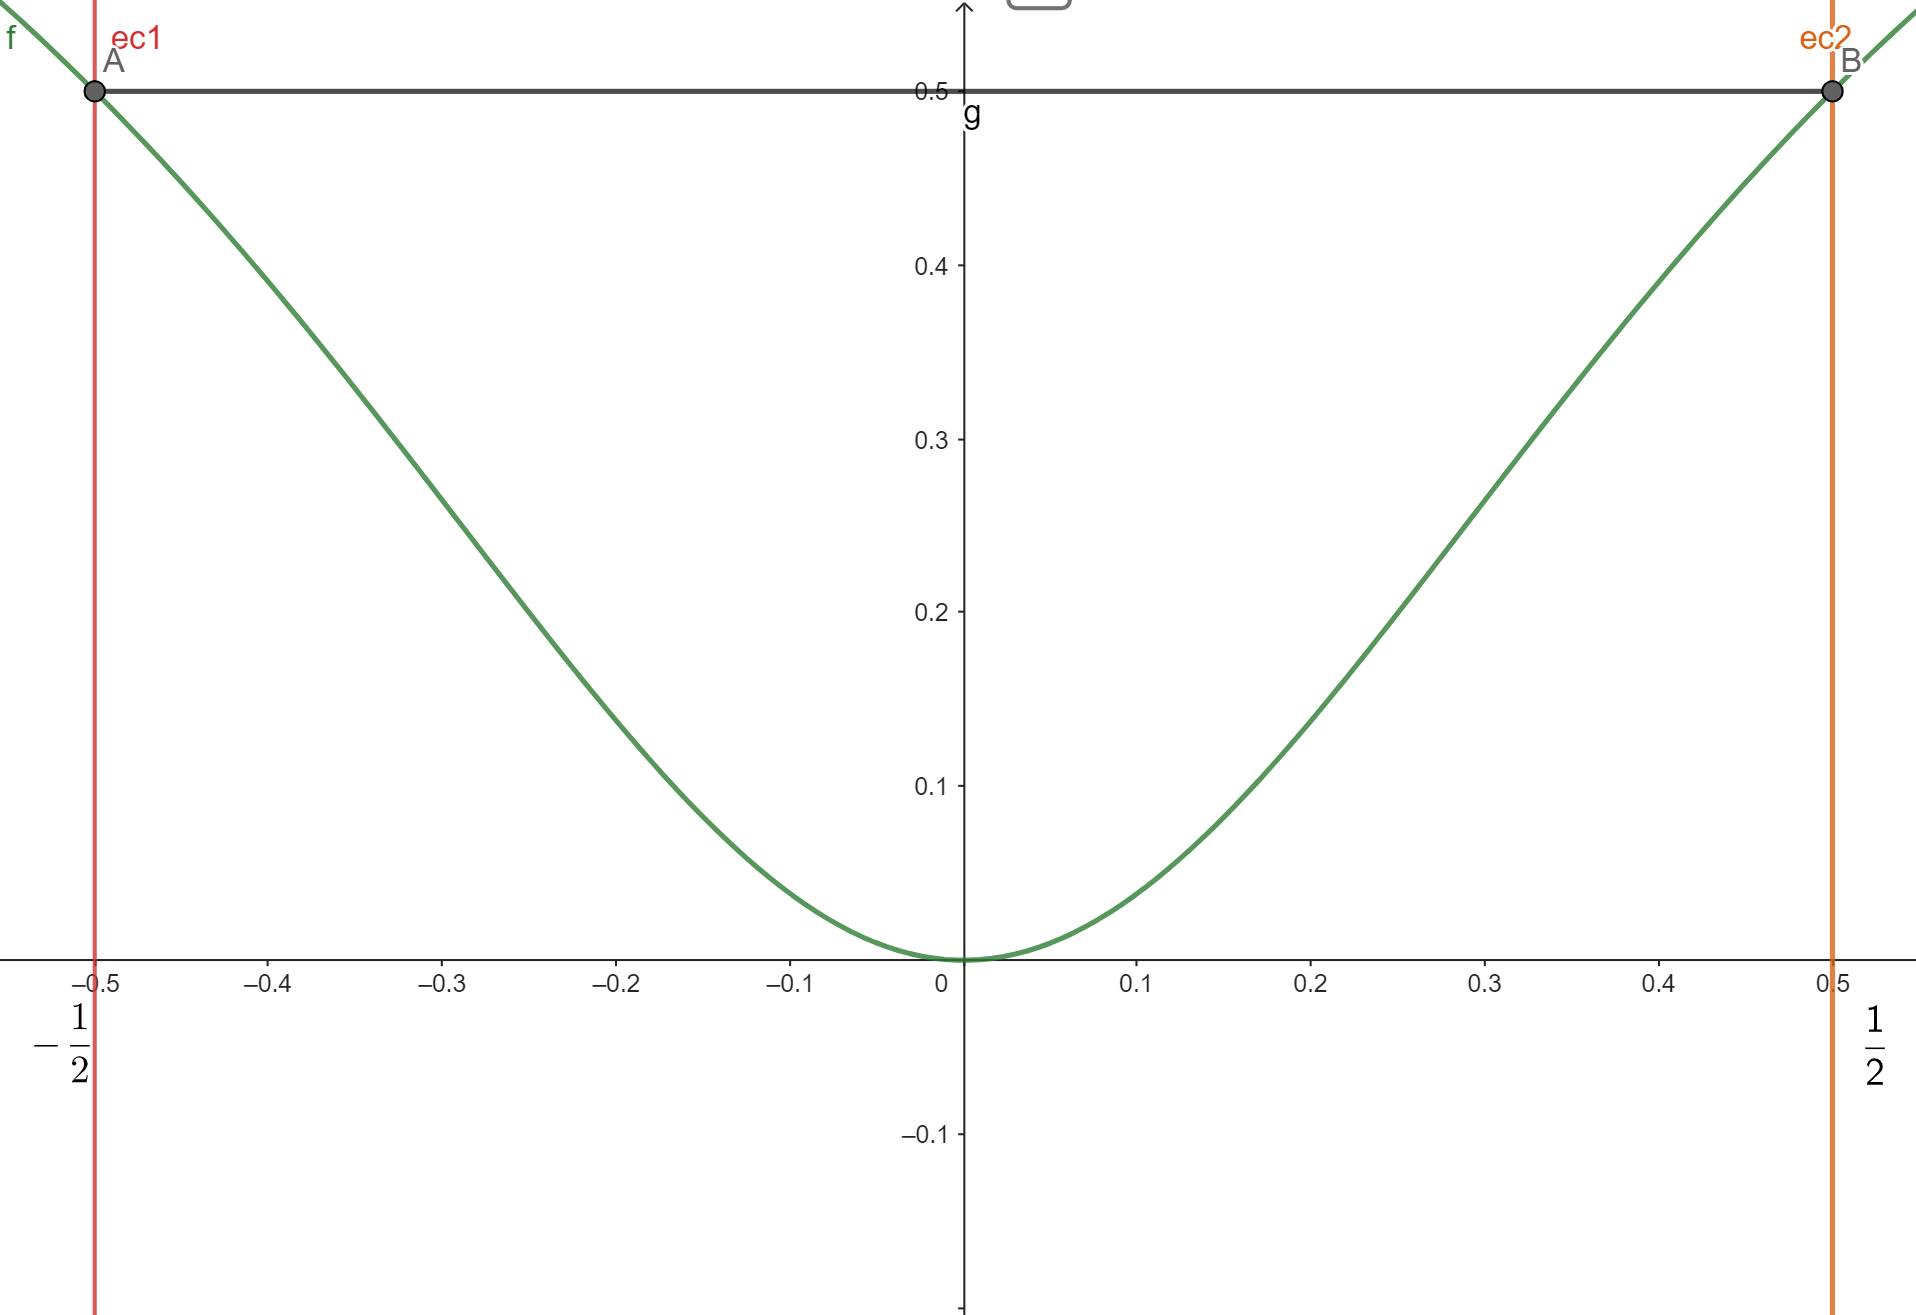
\includegraphics[scale=10]{imagenes/grafica 29-09.png}

$\lim_{n\to\infty}a_n=l\qquad$ si $\forall\varepsilon>0\exists n_0\in\mathbb{N}$ tal que si $n\ge n_0\rightarrow|a_n-l|<\varepsilon$

$f:A\subset\mathbb{R}\longrightarrow\mathbb{R}$

$x_0$ punto de acumulación de $A$.

$\lim_{x\to x_0}f(x)=l$ si $\forall\varepsilon>0\exists\delta>0$ tal que si $|x-x_0|<\delta\longrightarrow|f(x)-l|<\varepsilon$


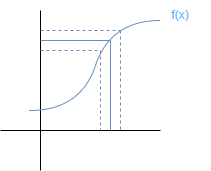
\includegraphics{"imagenes/grafica 18_10.png"}

$\lim_{x \to x_0}f(x)\neq l$ si $\exists\varepsilon>0$ tal que $\forall\delta>0\exists x_\delta$ tal que $|x-x_0|<\delta$ y $\left|f(x_\delta)-l\right|>\varepsilon$

El límite si existe, es único.
\begin{itemize}[label=\color{red}\textbullet, leftmargin=*]
	\item \color{lightblue}Demostración
\end{itemize}
Supongamos que: 

$l_1=\lim_{x\to x_0}f(x)\rightarrow\forall\varepsilon>0\exists\delta_1$ tal que $|x-x_0|<\delta_1\longrightarrow\boxed{|f(x)-l_1|<\varepsilon}$

$l_2=\lim_{x\to x_0}f(x)\rightarrow\forall\varepsilon>0\exists\delta_2$ tal que $|x-x_0|<\delta_2\longrightarrow\boxed{|f(x)-l_2|<\varepsilon}$

$|l_1-l_2|=|l_1-f(x)+f(x)-l_2|\le |l_1-f(x)|+|f(x)-l_2|\le\varepsilon+\varepsilon=2\varepsilon$

$|x-x_0|<\delta\coloneq\min\{\delta_1,\delta_2\}\longrightarrow$ (1) y (2) se cumplen.

$\begin{array}{l}
	\lim_{x\to x_0}f(x)=l\rightarrow\forall\varepsilon>0\:\exists\,\delta\text{ tal que }|x-x_0|<\delta\longrightarrow|f(x)-l|<\varepsilon\\
	\lim_{x\to x_0^+}f(x)=l\rightarrow\forall\varepsilon>0\:\exists\,\delta\text{ tal que }0<x-x_0<\delta\longrightarrow|f(x)-l|<\varepsilon\\
	\lim_{x\to +\infty}f(x)=l\rightarrow\forall\varepsilon>0\:\exists\,\delta\text{ tal que }x\ge k\longrightarrow|f(x)-l|<\varepsilon\\
	\lim_{x\to x_0}f(x)=+\infty\qquad(-\infty, k)
\end{array}$

$f(x)=\mathrm{e}^{\frac{1}{x}}\sin\left(\dfrac{\pi}{x}\right)$

\begin{tikzpicture}[baseline=(current bounding box.center)]% function
	\begin{axis}[xlabel=x,ylabel=y, axis lines=center, legend pos=north west]
		\addplot[lightblue, samples=150, domain=-1:2] {e^x};
		\legend{$e^x$};
	\end{axis}
\end{tikzpicture}\qquad$\begin{array}{l}
\lim_{x\to0^+}\mathrm{e}^{\frac{1}{x}}=+\infty\\
\lim_{x\to0^-}\mathrm{e}^{\frac{1}{x}}=0
\end{array}$

$\lim_{x\to0^+}\mathrm{e}^{\frac{1}{x}}\sin\left(\dfrac{\pi}{x}\right)$ no existe

\hrule

$\underset{a}{I}\xrightarrow[\rightsquigarrow]{f}\underset{f(a)}{\mathbb{R}}\supset J\xrightarrow{g}\mathbb{R}$

$f(I)\subset J$

$x\rightsquigarrow\boxed{f(x)}\in J\rightsquigarrow g(f(x))$\\
$\begin{rcases}
	f\text{ continua en }a\\
	g\text{ continua en }f(a)
\end{rcases}\longrightarrow g\circ f$ es continua en $a$

$\begin{array}{l}
	\lim_{x\to a}f(x)=f(a)\qquad\forall\:\varepsilon>0\,\exists\,\delta>0\text{ tal que si }|x-a|<\delta\text{ entonces }\left|f(x)-f(a)\right|<\varepsilon=\delta_2\\
	\lim_{y\to f(a)}g(y)=g(f(a))\qquad\forall\:\varepsilon>0\,\exists\,\delta_2>0\text{ tal que si }|y-f(a)|<\delta_2\text{ entonces }\left|g(y)-g(f(a))\right|<\varepsilon\\
	\lim_{x\to a}(g\circ f)(x)=g\circ f(a)\\
	\forall\,\varepsilon>0\exists\,\delta^*>0\text{ si }|x-a|<\delta^*\longrightarrow\bboxed{\left|g\left(f(x)\right)-g\left(f(a)\right)\right|}
\end{array}$

Fijado $\varepsilon>0\longrightarrow\exists\,\delta_2>0$ que cumple (2).\\
En (1) tomamos $\varepsilon\coloneq\delta_2\longrightarrow\exists\,\delta^*>0$ tal que $|x-a|^2<\delta$

\begin{center}
	\includegraphics[scale=0.5]{"imagenes/Gráfica 20-10"}
\qquad
\includegraphics{"imagenes/Gráfica2 20-10"}
\end{center}

$\begin{array}{l}
	f'(a)=\lim_{x\to a}\dfrac{f(x)-f(a)}{x-a}=\left\{h=x-a\right\}=\lim_{h\to0}\dfrac{f(a+h)-f(a)}{h}\\
	f'(a)\simeq\dfrac{f(a+h)-f(a)}{h}
\end{array}$

$f:I\longrightarrow\mathbb{R}\quad a\in I$

$f$ es derivable en $a\longrightarrow f$ es continua en $a$ \[\cancel{\Longleftarrow} \]
\textcolor{lightblue}{\underline{Ejemplo}}

$\begin{array}{l}
	f(x)\begin{cases}
	x^2\sin\left(\dfrac{1}{x}\right) & x\neq0\\
	0 & x=0
\end{cases}\\
\lim_{x\to0}x^2\cdot\sin\left(\dfrac{1}{x}\right)=0=f(0)\text{ continua}\\
\begin{aligned}
	x\neq0\quad f'(x)&=2x\cdot\sin\left(\dfrac{1}{x}\right)+x^2\cos\left(\dfrac{1}{x}\right)\cdot\dfrac{-1}{x^2}\\
	& =2x\cdot\sin\left(\dfrac{1}{x}\right)-\cos\left(\dfrac{1}{x}\right)
\end{aligned}\\
f'(0)=\lim_{x\to0}\dfrac{f(x)-f(0)}{x-0}=\lim_{x\to0}\dfrac{x^{\cancel{2}}\cdot\sin\left(\frac{1}{x}\right)}{\cancel{x}}=\lim_{x\to0}x\cdot\sin\left(\dfrac{1}{x}\right)=0\\
\lim_{x\to0}f'(x)=\lim_{x\to0}\underbrace{2x\cdot\sin\left(\dfrac{1}{x}\right)}_0-\cos\left(\dfrac{1}{x}\right)\text{ no existe}\\
f'(x)=\begin{cases}
	2x\sin\left(\dfrac{1}{x}\right)-\cos\left(\dfrac{1}{x}\right) & x\neq0\\
	0 & x=0
\end{cases}\\
\text{No es continua en $x=0$}
\end{array}$

\begin{center}
	Derivable $\Longrightarrow$ continua
\end{center}

$\begin{array}{l}
	f'(a)=\lim_{x\to a}\dfrac{f(x)-f(a)}{x-a}\longrightarrow\forall\,\varepsilon>0\exists\,\delta>0\text{ tal que }|x-a|<\delta\text{ entonces }\left|\dfrac{f(x)-f(a)}{x-a}-f'(a)\right|<\varepsilon\\
	\lim_{x\to a}f(x)=f(a)\\
	\forall\,\varepsilon>0\:\exists\,\delta>0\text{ tal que si}|x-a|<\delta\longrightarrow|f(x)-f(a)|<\varepsilon\\
	\left|\dfrac{f(x)-f(a)}{x-a}-f'(a)\right|<\varepsilon\\
	|f(x)-f(a)-f'(a)\cdot(x-a)|<\epsilon\cdot|x-a|\\
	\begin{aligned}
		|f(x)-f(a)|&=|f(x)-f(a)-f'(a)\cdot(x-a)+f'(a)\cdot(x-a)|\\
		&\le|f(x)-f(a)-f'(a)\cdot(x-a)|+|f'(a)|\cdot|x-a|\\
		&\le\varepsilon\cdot|x-a|\\
		&=|x-a|\cdot\left(\varepsilon+|f'(a)|\right)<\delta\cdot\left(\varepsilon+|f'(a)|\right)=\varepsilon^*
	\end{aligned}\\
	\varepsilon^*=\delta\cdot(\epsilon-|f'(a)|)\longrightarrow\dfrac{\epsilon^*}{\delta}=\left(\varepsilon+|f'(a)|\right)\longrightarrow\varepsilon\coloneq\bboxed{\dfrac{\varepsilon^*}{\delta}-|f'(a)|>0}
\end{array}$
\begin{center}
	\begin{tikzpicture}
		\begin{axis}[axis lines=center]
			\addplot[lightblue, samples=150, domain=1:3] {-1+x};
			\addplot[lightblue, samples=150, domain=-1:1] {1-x};
		\end{axis}
	\end{tikzpicture}
\end{center}
$\begin{array}{l}
	\arcsin\left(\sin(x)\right)=x\\
	\arcsin'(\sin(x))\cdot\cos(x)=1\longrightarrow y=x^{\sin(x)}\qquad\log(y)=\sin(x)\cdot\log(x)
\end{array}$

$f'(a)=\lim_{x\to a}\dfrac{\overset{+}{f(x)-f(a)}}{\underset{+}{x-a}}>0$

\begin{center}
	\includegraphics{"imagenes/Gráfica 27-10"}
	\qquad
	\includegraphics{"imagenes/Gráfica2 27-10"}
\end{center}


$\begin{array}{l}
	f'(x)=0\\
	f:[a,b]\longrightarrow\mathbb{R}\text{ continua y derivable }(a,b)
\end{array}$

Compacto (cerrado + acotado) $\longrightarrow$ dimensión finita

$\begin{array}{l}
	f(x)=\dfrac{x^2-2x+1}{x^2+2x+2}\qquad\mathrm{Dom}(f)=\mathbb{R}\\
	\begin{aligned}
		f'(x)&=\dfrac{(2x-2)(x^2+2x+2)-(x^2-2x+1)(2x+2)}{(x^2+2x+2)^2}\\
		&=\dfrac{\cancel{2x^3}+2x^2+2x-2x^2-4x-4-(2x^3+2x^2-4x^2-4x+2x+2)}{(x^2+2x+2)^2}\\
		&=\dfrac{4x^2+2x-6}{(x^2+2x+2)}=\dfrac{2(2x^2+x-3)}{(x^2+2x+2)}=\dfrac{2\cdot2\left(x+\frac{3}{2}\right)\cdot(x-1)}{(x^2+2x+2)^2}
	\end{aligned}\\
	\lim_{x\to+\infty}\dfrac{x^2-2x+1}{x^2+2x+2}=\lim_{x\to+\infty}\dfrac{x^2\cdot\left(1-\cancelto{0}{\frac{2}{x}}+\cancelto{0}{\frac{1}{x^2}}\right)}{x^2\cdot\left(1+\cancelto{0}{\frac{2}{x}}+\cancelto{0}{\frac{2}{x^2}}\right)=1}
\end{array}$
\begin{center}
	\begin{tikzpicture}% function
		\begin{axis}[xlabel=x,ylabel=y, axis lines=center, width=0.9\textwidth]
			\addplot[lightblue, samples=400, domain=-30:30] {(x^2-2*x+1)/(x^2+2*x+2)};
			\addplot[lightblue, dashed, domain=-30:30, line width=1.5pt] {1};
		\end{axis}
	\end{tikzpicture}
\end{center}
\textcolor{lightblue}{\underline{Ejercicio A. Examen Enero 2023}}

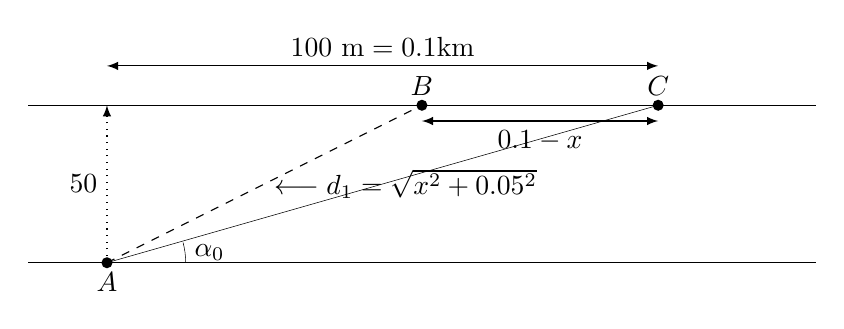
\begin{tikzpicture}[baseline=(current bounding box.center)]
	\draw (0,0) -- (10, 0);
	\draw (0,-2) -- (10,-2);
	\fill (1,-2) circle (2pt) node[below] {$A$};
	\fill (5,0) circle (2pt) node[above] {$B$};
	\fill (8,0) circle (2pt) node[above] {$C$};
	\draw[-latex, dotted] (1,-2) -- (1, 0) node[midway, left] {50};
	\draw[dashed] (1,-2) -- (5,0) node[midway, right] {$\longleftarrow d_1=\sqrt{x^2+0.05^2}$};
	\draw[latex-latex] (1,0.5) -- (8,0.5) node[midway, above] {$100\text{ m}=0.1 \text{km}$};
	\draw[latex-latex] (5,-0.2) -- (8,-0.2) node[midway, below] {$0.1-x$};
	\draw[line width=0.2pt] (1,-2) -- (8,0);
	\draw[line width=0.2pt] (2,-2) arc (0:15:1) node[midway,right] {$\alpha_0$};
\end{tikzpicture}\qquad
$\begin{array}{l}
	\text{nadar}\longrightarrow 3\text{ km/h}=\dfrac{3}{60}\text{ km/min} =\dfrac{1}{20}\text{ km/min}\\
	\text{andar}\longrightarrow 5 \text{ km/h}= \dfrac{5}{60}\text{ km/min} = \dfrac{1}{12}\text{ km/min}\\
	T=\dfrac{e}{v}\\
	T(x)=\dfrac{\sqrt{x^2+0.05^2}}{\frac{1}{20}}+\dfrac{(0,1-x)}{\frac{1}{12}}\\
	T'(x)=0\\
	x\in [0,0.1]
\end{array}$

\begin{center}
	\begin{tikzpicture}% function
		\begin{axis}[xlabel=x,ylabel=y, axis lines=center, width=0.5\textheight]
			\addplot[lightblue,samples=150, domain=-2:3] {e^x};
		\end{axis}
	\end{tikzpicture}
\end{center}

$\begin{array}{l}
	f(x)\qquad x_0\longrightarrow f(x_0),f'(x_0),\dots,f^{n)}(x_0)\\
	f(x)\simeq P_n(x)=f(x_0)+\dfrac{1}{1!}f'(x_0)(x-x_0)+\dfrac{f''(x_0)}{2!}(x-x_0)^2+\cdots+\dfrac{f^{n)}(x_0)}{n!}(x-x_0)^{n}\\
	x_0=0\longrightarrow\text{ McLaurin}\\
	\mathrm{Error}(X)=\dfrac{f^{n+1)}(c)}{(n+1)!}(x-x_0)^{n+1}\\
	\begin{array}{r|l}
		c\in(x_0,x) & c\in(x,x_0)\\
		x>x_0 & x<0
	\end{array}\\
	\underset{\sin(x)\equiv x\quad(x\to0)}{\lim_{x\to0}\dfrac{x-\sin(x)}{x^3}}=\lim_{x\to0}\dfrac{x-\left(x-\frac{x^3}{3!}+\frac{x^5}{5!}-\cdots\right)}{x^3}=\lim_{x\to0}\dfrac{\frac{x^3}{3!}-\frac{x^5}{5!}+\cdots}{x^3}=\lim_{x\to 0}\dfrac{1}{3!}-\left[\cancelto{0}{\dfrac{x^2}{5!}}+\cancelto{0}{\dfrac{x^4}{2!}}+\cdots\cancelto{0}{=}\cdots\right]=\bboxed{\dfrac{1}{6}}\\
	\underset{\boxed{x_0=0}}{\sin(x)}\simeq x-\dfrac{x^3}{6}+\dfrac{x^5}{5!}+\cdots+\mathrm{error}\\
	\mathrm{Error}\left(\dfrac{1}{2}\right)=\dfrac{1}{4!}\cdot{\Large e}^c\cdot\left(\dfrac{1}{2}-0\right)^4=\dfrac{1}{24}\cdot{\Large e}^c\dfrac{1}{2^4}\\
	\begin{tikzpicture}[baseline=(current bounding box.center)]% function
		\begin{axis}[axis lines=center, ymin=-1]
			\addplot[lightblue, samples=150, domain=-1:1] {e^x};
			\draw[lightblue] (axis cs:0.5,0) -- (axis cs:0.5, 1.6487212707001);
			\draw[lightblue] (axis cs:0.25,0.1) -- (axis cs:0.25,-0.1) node[below] {$c$};
			\fill[lightblue] (axis cs:0,1) circle (2pt);
		\end{axis}
	\end{tikzpicture}\qquad \begin{array}{l}
	1<e^c<e^{\frac{1}{2}}\le 2\\
	\left|\mathrm{Error}\left(\dfrac{1}{2}\right)\right|\le\dfrac{1}{3^4}\cdot2\cdot\dfrac{1}{3^4}=\dfrac{1}{2^4}\cdot\dfrac{1}{2^3}=0.0026042
	\end{array}
\end{array}$

$\begin{array}{r}
	\left.\begin{array}{r}
		(x_1,f(x_1))\\
		f'(x_1)
	\end{array}\right\}\longrightarrow y-f(x_1)=f'(x_1)(x-x_1)\\
	\begin{cases}
		y=f(X_1)+f'(x_1)(x-x_1)\\
		y=0
	\end{cases}\\
\end{array}$\\
$	\begin{aligned}
	f(x_1)+f'(x_1)(x-x_1)=0\longrightarrow f'(x_1)(x-x_1) &=-f(x_1)\\
	x-x_1&=\dfrac{-f(x_1)}{f'(x_1)}
\end{aligned}\longrightarrow x=x_1-\dfrac{f(x_1)}{f'(x_1)}$

\begin{center}
	\includegraphics[width=0.5\linewidth]{"imagenes/Gráfica 03-11"}
\end{center}

\end{document}
